\documentclass{article}

%Header + title info
\title{Honors Thesis\\(Draft)}
\author{Gideon Moore}

%Bibliography info
\usepackage[style = authoryear, backend = bibtex]{biblatex}
\addbibresource{Sources.bib}

%Graphics info
\usepackage{graphicx}

%Misc packages
\usepackage{microtype}
\usepackage[includeheadfoot]{geometry}
\usepackage{booktabs}
\usepackage{blindtext}
\usepackage{amsmath}
\usepackage{amsfonts}
\usepackage{setspace} %For line spacing
\usepackage{xcolor} %For commenting visibly

%Header (MUST BE LOADED AFTER GEOMETRY)
\usepackage{fancyhdr}
\pagestyle{fancy}
\lhead{Honors Thesis (Draft)}
\chead{Gideon Moore}
\rhead{March 2018}

\usepackage{subcaption} %For subfigures



\begin{document}
	{\setstretch{1} \maketitle}
	
	\setstretch{2}
	
	\section*{Abstract}
	
	\blindtext
	
	\pagebreak
	
	\section{Introduction}
	
	From 2000 to 2015, total undergraduate enrollment rose by 30\% from 13.2 to 17 million students \parencite{mcfarland2017}. Meanwhile, the real quantity of outstanding student debt tripled from \$340 billion to more than \$1.3 trillion over the same period \parencite{feiveson2018}.
	
	Traditional models of investment would suggest financing methodology would not change consumer behavior--for a given student, whether they finance their education with debt or existing capital would not change their consumption decisions. However, empirically this is not the case. A survey by Nellie Mae suggests that one in six loan recipients have changed their career plans due to their debt obligation \parencite{baum2003}. This survey contained only those who had not yet defaulted on their debt; as defaulters were heavily affected by debt, the true number is likely greater. \textcite{minicozzi2005} finds that men who take on more undergraduate debt take jobs with higher initial wages but lower year-over-year wage growth, again suggesting a real impact of what should be a purely accounting-based change. 
	
	A debt subsidy could theoretically create an income effect, however even an extremely generous program promising zero interest on student debt would only increase students' income by around \$50 per year per thousand dollars borrowed--a fraction of the expected lifetime earnings of a college attendee. Thus, it is unlikely the income effect from this subsidy would be able to explain any of the behavior outlined above.
	
	An alternate explanation as to why debt would change students' behavior is that students may be ``debt averse,'' meaning that the act of holding debt has a negative impact on students' utility independent of any impact that debt may have on consumption. This would cause students to pay off debt more quickly than would be efficient, ``consuming'' through paying off debt ahead of schedule. Students who are minorities, low-income, or first generation are especially susceptible to this phenomenon \parencite{burdman2005, field2009, callender2005}. 
	
	One frequent explanation for this phenomenon is risk aversion. Given student debt is uniquely difficult to disperse, the consequences for default can be catastrophic. Thus, as students take on more debt, they risk failing to pay back their loans. It is rational, then, to gravitate to higher paying, more stable careers which could bring a higher risk of insolvency. 
	
	The most relevant study on debt aversion is by \textcite{field2009}. In her trial, New York University law students were randomly assigned either loan- or grant-based aid. The students assigned loans were told that their debt would be forgiven upon entry into a public service sector. Similarly, students given grants were told that, if they did \emph{not} enter the public service sector, they would be obligated to repay their grants. The two programs were designed to be financially identical--they differed only in the framing of whether the student was ``in debt.'' However, the author found that the students who were given the debt-based aid were significantly more likely to choose the high-wage, non-public-service position than their counterparts receiving grant-based aid. Given the aid packages are financially identical, the authors conclude this likely derives from some negative socio-psychological impact of carrying debt.
	
	In an ideal world, we could answer the question of debt and employment through regressing some measure of career choice on debt level. However, endogeneity issues make this solution infeasible. Given students choose to take debt based on expectations of their future earnings, there exists a reverse-causal effect from career to debt. Therefore, we require some sort of random assignment in order to accurately infer causality. 
	
	The focus of this paper is to determine whether increases in debt lead students to change their fields of study and eventually career choices. While prior work in the literature has largely focused on policy changes within a single institution, I hope to create a more representative picture of the nation as a whole using data from the National Longitudinal Survey of Youth. In 2006, the United States raised the cap for Stafford Loans for freshmen and sophomores, creating a natural experiment wherein the students before the policy change were more limited in their access to debt than the students after the shift.
	
	[RESULTS RESULTS RESULTS]
	
	\section{Literature Review}
	
	The current central paper of the literature is \textcite{rothstein2011}, which uses the introduction of a ``no loans'' policy at prestigious private college ``Anon U''--implied to be Princeton University--as a natural experiment on the enrolled students. The authors use a function of expected family contribution as an instrument for the impact of the policy, discovering that an additional \$10,000 of student debt leads students to reduce employment in the non-profit and education sectors by 5.2\% and reduce employment in low-wage sectors generally by 5.7\%. This is further corroborated by an expected \$2,000 bump in wages per \$10,000 of debt. The authors also suggest increased debt shifts students towards more ``employable'' majors over what they describe as ``consumption'' majors. The main shortfall of this paper which I hope to correct is that Princeton students are not representative of the general population -- as of 2017, nearly 60\% of students at Princeton came from families in the top 10\% of Americans by income \parencite{aisch2017}. Other papers have examined similar phenomena in more specialized and similarly wealthy fields, finding that increased debt leads both dentists and lawyers to accept higher-paying jobs in disproportionately private practices \parencite{nicholson2015, field2009}.
	
	One suggestion for this form of behavior is a phenomenon called ``debt aversion,'' where borrowers are less inclined to take and carry debt than a traditional model would indicate. \textcite{burdman2005} finds many non-income factors can influence whether students choose to borrow to attend school. One of the most influential factors she found was parental attitudes towards loans, suggesting that students whose parents were debt averse were more likely to be debt averse themselves. \textcite{callender2005} find that low-income and minority students are significantly less likely to borrow, regardless of their field of study. However, \textcite{eckel2007} find that students who are debt averse are not significantly less likely to have borrowed to attend school, suggesting that we can expect to see debt aversion in our sample. 

	\section{Structural Model}
	
	\begin{figure}
		\centering
		\caption{Illustration of Structural Model}
		\label{struc}
		\includegraphics[width = 0.8\textwidth]{Images/ModelSketch}
	\end{figure}

	Consider a two-stage consumption model. Individuals consume in period one entirely through borrowing against period two earnings, labeled as $B$. In period one agents choose to pursue a higher-paying career path $H$ or a lower-paying career path $L$. Consumption in period two is composed of two parts, less the quantity borrowed in period one. First, $C$, non-monetary utility from the chosen career path; consider the value of altruism for working in a non-profit or the value of expression for working as an artist. The second consumption parameter in time two is monetary salary, denoted $H$ and $L$ for the higher- and lower-paying careers respectively.
	
	When taking career $L$, there is a risk $p$ of defaulting on your loan, in which case your monetary compensation for the period is reduced to zero, leaving only non-monetary compensation $C$. We assume that \emph{ceteris paribus} larger loans are more difficult to repay; thus, $p$ is a function increasing in $B$. Finally, there is some discount rate $r$ for the money borrowed in period one. This $r$ will favor the present, as we are examining interest-free loans for our students. This yields the following two utility functions for a risk-neutral consumer: 
	\begin{align}
	\mathbb{E}\left[U_H(B)\right] &= B + H - (1 - r)B \label{highu}\\
	\mathbb{E}\left[U_L(B)\right] &= B + C + p(B) \times L - (1 - r)B \label{lowu}
	\end{align}
	
	Note that students choosing career $L$ over career $H$ suggests that equation \ref{highu} is greater than equation \ref{lowu}. Some algebra yields the following equivalence relationship: 
	$$\mathbb{E}\left[U_L(B)\right] - \mathbb{E}\left[U_H(B)\right] > 0 \iff p(B) > \frac{H - C}{L} \label{choicecon}$$ 
	Thus, there are five factors that could shift students from $H$ to $L$:
	\begin{itemize}
		\singlespacing
		\item A decrease in $H$
		\item An increase in $C$
		\item An increase in $L$
		\item A change in the definition of $p$
		\item An increase in $B$, as $p'(B) < 0$
	\end{itemize}

	The above model is deterministic for any given student; given a fixed $H, C, L, p,$ and $B$ they will always choose the same career. Moreover, for simplicity, we allow $H, L$, and $p$ to be constant across all students, representing access to similar credit and labor markets. However, there exists idiosyncratic variation in $C$ between students; student $i$ may derive great utility from career $L$, while student $j$ may not care for $L$ at all.

	Note that for each student there exists some $B^*$ such that they are indifferent between $H$ and $L$. Suppose there exists some global upper bound on borrowing $\bar{B}$ which is binding for both those on career paths $H$ and $L$. When $\bar{B}$ is increased as in figure \ref{struc}, this will cause some--but not all--students to shift career from $L$ to $H$ as $\bar{B}$ may shift to be greater than $B^*$ for some subset of students. Given students before and after this change are comparable, we could treat this shift as a natural experiment, providing each student after the shift with an additional $\Delta\bar{B}$ debt burden. 
	
	\textcolor{darkgray}{[COMMENT: I've been thinking about the welfare implications of this model for a while and haven't really reached a conclusion yet. It's clear there's a societal cost to these subsidized loans: $(1 - r)B$ is all government expenditure. Further, it seems as though shifting from line $H$ to line $L$ causes $C$ to be lost to society; while the wage difference $(H - L)$ is a transfer from firms, and so neither creates nor destroys welfare in perfect competition, the loss of $C$ appears to be a societal loss. Thus, while loans can be positive for equality, it seems like they may be quite costly to society. Unfortunately these costs are difficult to quantify since $C$ is a subjective value. The paper which inspired this model \parencite{abraham2018} suggests that income based repayment plans can provide the equality benefits without changing career choices, so that could be a good point of reference.]}

	\section{HERA and Subsidized Student Loans}
	
	I borrow my identification strategy from \textcite{lucca2018} who examine how increased Federal subsidized credit lines impact university tuition. In 2006, the Higher Education Reconciliation Act (HERA) increased subsidized borrowing caps for the first time in fourteen years. Freshmen received boosts from \$2,625 to \$3,500 per year, while sophomores received a greater boost from \$3,500 to \$4,500 per year. Caps for older students remained static at \$5,500. While HERA also increased the availability of unsubsidized credit, Lucca and his coauthors make a compelling argument that the increase in unsubsidized loan caps had a middling effect at best on uptake for unsubsidized loans. Students who increase unsubsidized borrowing under the program shift would have to meet two criteria: first, the students would have to be well off enough to not qualify for a wholly subsidized program, and second, the students still chose to take advantage of their whole program allowance. The authors find that fewer than 1\% of the students in their sample met both of these criteria.
	
	The act became effective during early summer 2007, meaning students had plenty of time to take advantage of the new rates before the fall semester. Thus, there is a clean break between the students with and without the lower credit limit moving from academic year 2006-07 and 2007-08.
	
	The authors also provide evidence that the subsidized loan cap had previously been binding. Figure \ref{luc} contains histograms of student-level loan quantities before and after the HERA shift from the New York Fed/Equifax Consumer Credit Panel. Figure \ref{luc06} has a clear mode of \$2,625, the exact subsidized cap for freshmen pre-HERA, and a secondary mode of \$3,500, the subsidized cap for sophomores. Compare this with figure \ref{luc07}, which has modes at \$3,500 and \$4,500, the post-HERA caps for freshmen and sophomores, respectively. Further note that both graphs contain clusters at \$5,500, the constant cap for upperclass students, again suggesting the binding nature of the subsidized loan cap. 
	
	
	\begin{figure}
		\centering
		\caption{Student Loan Frequencies From NY Fed CCP/Equifax Panel as Presented in \textcite{lucca2018}.}
		\label{luc}
		\begin{subfigure}{0.49\textwidth}
		\centering
		\caption{Student Loan Frequencies 2006-2007}
		\label{luc06}
		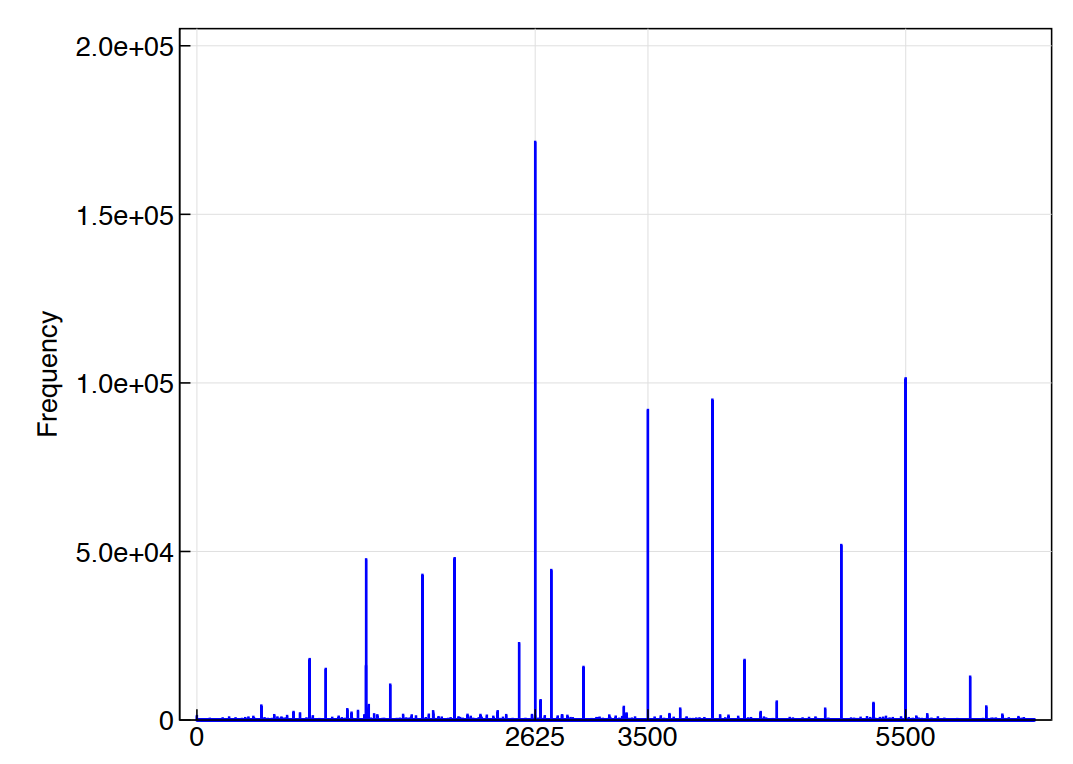
\includegraphics[width = \linewidth]{Images/Lucca6a.png}
		\end{subfigure} 
	\begin{subfigure}{0.49\textwidth}
		\centering
		\caption{Student Loan Frequencies 2007-2008}
		\label{luc07}
		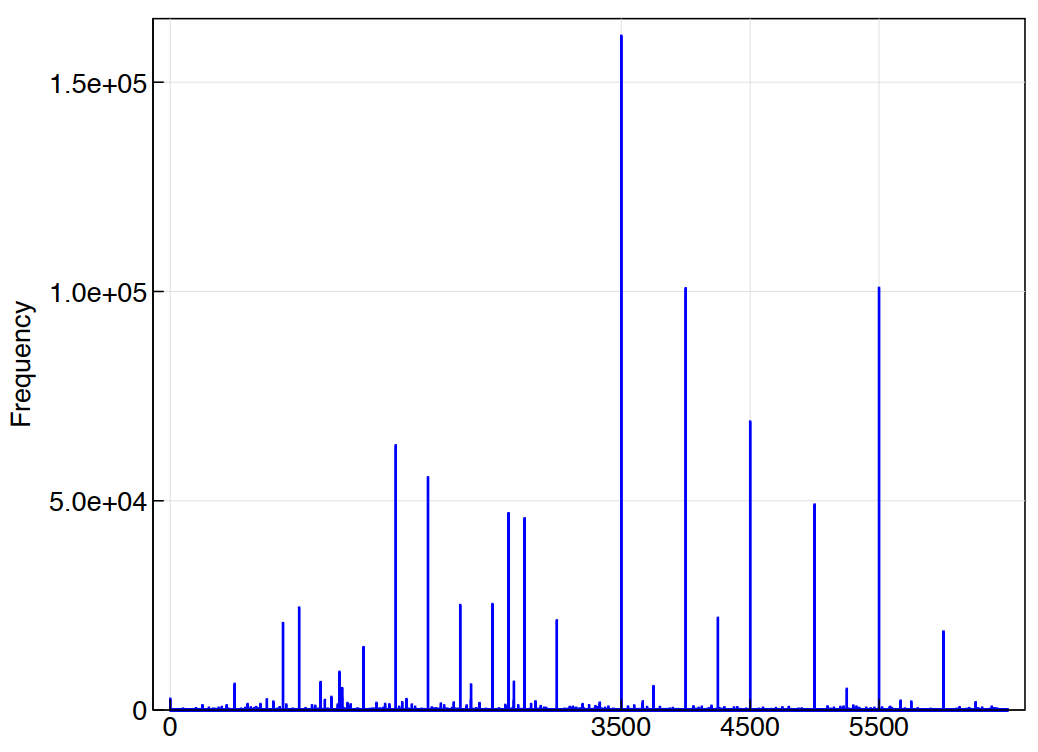
\includegraphics[width = \linewidth]{Images/Lucca6b.png}
		\end{subfigure}
	\end{figure}
	
	\section{Data}
	
	For my paper I use data from the National Longitudinal Survey of Youth '79 Children and Young Adults (NLSY79 CYA). A follow-up to the original National Longitudinal Survey of Youth '79, the CYA surveys the original respondents' children semiyearly from birth until the present day. Thus, we have respondents across the entire age spectrum during the implementation of the policy, allowing us to observe time-varying trends in debt acquisition and career choice. 
	
	\begin{figure}
		\centering
		\caption{Distribution of Parental Income}
		\label{incDist}
		\includegraphics[width = 0.9\textwidth]{../Analysis/Charts/Output/parIncDist}
	\end{figure}
	
	The benefits of the CYA data over the Princeton data from \textcite{rothstein2011} are several. First, the NLSY is designed to focus on lower income households rather than Anon U's much wealthier sample. As visible in figure \ref{incDist}, 20\% of students come from households below the federal poverty line, as opposed to 10\% nationally. Second, the students in this survey attend a much broader range of colleges than those in the Rothstein data set. As the students who are accepted into prestigious universities such as Anon U are by definition selected, they \emph{cannot} be representative of the general American college-bound population. Third, the CYA surveys students both about their finances and about their career aspirations at each step of the process. Thus, not only can I track student outcomes after graduation, I am able to plot students' intentions over time, tracking variables such as intended major during their time at school. This provides a more interesting, nuanced panel as we can see how students' intentions evolve as their access to credit changes. Finally, with data from several different colleges, we can examine how college traits interact with student debt and career outcomes. 
	
	\begin{figure}
		\centering
		\caption{Distribution of Loan Size}
		\label{loanDist}
		\includegraphics[width = 0.9\textwidth]{../Analysis/Charts/Output/loanDist}
	\end{figure}
	
	One drawback of the CYA data set is that, as a survey, many of the figures are less precise than those in other sets. For example, when asked about their level of debt, the vast majority of responses are rounded numbers. While useful for qualitative analysis, this makes it difficult to assess data granularly as done by \textcite{lucca2018} in figure \ref{luc}. Fortunately, because they have a nationally representative dataset, there is no reason to believe their results would differ with our sample. Indeed, as our sample is of lower income relative to the general population, I would argue that subjects are bound more strongly by the policy as for many students federal loans may be their only option for college financing. In addition, as visible in figure \ref{loanDist}, we can see that 85\% of students received \$10,000 or less in debt, suggesting an additional \$1,000 would be meaningful relative to their overall quantity. 
	
	Because of the connection between the CYA and original NLSY79, we can import very rich background information for each of our participants. Specifically, for each student we can identify parental income for the year in question among other background traits inherited from parents.
	
	\section{Statistical Model}
	
	Our data set is a collection of seniors surveyed on even years between 2000 and 2016. If possible, we would hope to model some career outcome $Y$ according to the following equation: $$Y = \beta_0 + \beta_1 \ln(\mbox{debt})_{it} + \vec{\xi}^T \vec{\mbox{demographics}}_i + \epsilon_{it}$$ In this model, $Y$ could take one of several values, such as major choice, career choice, or salary. 
	
	Our first model will place major choice on the left hand side. I believe this to be the most novel outcome of interest, as few datasets have this level of resolution on their observations. Here I can use a random variable logit model to place students into one of six bins: humanities, STEM, Social Science, Professional, Business, and Pre-Grad. The specifications of these bins can be found in the appendix, and we will adjust these bins later as a form of robustness testing. The distribution of students broken down by major is visible in figure \ref{majDist}.

	\begin{figure}
		\centering
		\caption{Breakdown of major in sample}
		\label{majDist}
		\includegraphics[width = 0.9\textwidth]{../Analysis/Charts/Output/majDist}
	\end{figure}
	
	Our second model will be examining students' career outcomes. This is the outcome most widely researched in the literature, such as in \textcite{rothstein2011} and \textcite{field2009}. Similar to the regression above, this would use a mixed logit model to examine whether increased debt pushes students into certain categories of career.
	
	Our final model will be directly examining students' final incomes. This is the most direct approach to measuring the impact of debt on choices; however, it may ignore factors such as career risk which would not be visible in simple income data.
	
	Unfortunately there exists reverse causality between debt and career choices; therefore, we must perform a two-stage least squares regression using exposure to the HERA credit increase as our instrumental variable in order to pseudo-randomly assign debt to our students. 
	
	We assume that outside of our random assignment, debt levels are dependent on parental resources, time trends, and demographic characteristics such as sex, race, and region of residence. As the time trend for debt levels may not be linear, we use dummies for each year to represent average debt within our sample for a given year. Further, we anticipate students taking out loans each semester; thus, those interviewed in the fall of their senior year would have less debt than those in the spring, so we include a semester dummy as well.
	
	The ideal first-stage model, then, would be: $$debt_i = \delta_0 + \delta_1 treatment_i + \delta_2 parIncome_i + \delta_3 fallSemester_i + \vec{\delta}^T i.year_i + \vec{\gamma}^T \vec{demographics}_i + \mu_i$$
	
	There exist two primary problems with this approach, however. The first is that debt is inherently left-censored. While students who take loans display some positive value, those who choose not to borrow display zero when they instead potentially chose some ``negative'' through investing their assets rather than borrowing. 
	
	The solution to this issue is to perform the first stage regression using a Tobit model rather than traditional OLS. This creates problems of its own however; as the Tobit is nonlinear, errors of projected values are not guaranteed to be uncorrelated. I therefore use a method suggested by \textcite{angrist2009} whereby the fitted Tobit values are used themselves as instruments for debt. 
	
	The second difficulty this model faces is that it is difficult to determine which students are ``treated,'' as not all students observed after the policy change received the additional credit. Since subsidized loans are targeted at low-income families, only students whose anticipated need is greater than the existing cap were subject to this increased credit line. 
	
	Anticipated need is equal to students' tuition payments minus their expected family contribution, or EFC. While we cannot observe students' true EFC, we can calculate an approximation using the Free Application for Federal Student Aid (FAFSA). Then, using this approximation, we are able to generate a measure of need and so determine who is affected by the policy shift. We then generate a dummy $atCap$ equal to 1 if a student's need is greater than the old borrowing limit and so are in our sample. 
	
	Thus, our final model for the first stage is as follows: $$debt_i = \delta_0 + \delta_1 treatmentSize_i + \delta_2 treatmentSize \times atCap + \delta_3 need + \delta_4 fallSemester + \vec{\delta}^T i.year + \vec{\gamma}^T \vec{demographics} + \mu_i$$ Given our model is correct, our coefficient of interest is $\delta_2$, the impact of being treated on those who were treated. Note we anticipate $\delta_1$ to be zero, as the policy should not impact those who are not in the targeted group.
	
	\textcolor{darkgray}{[COMMENT: Note this is where we run into problems--somehow $\delta_2$ does not end up being significant. I was surprised by this as we know from figure \ref{luc}, which used data directly from Fannie Mae, that this policy seems to have had a quite significant impact. This makes me think there's something we're not accounting for; potentially we need better controls for need or some better way to control for debt levels for the untreated students.]}
	
	
	\section{Results}
	
	\blindtext
	
	\section{Discussion}
	
	\blindtext
	
	\section{Conclusion}
	
	\blindtext

	\printbibliography
	
\end{document}